\chapter{\ifproject%
\ifcpe การทดลองและผลลัพธ์\else Experimentation and Results\fi
\else%
\ifcpe การประเมินระบบ\else System Evaluation\fi
\fi}

การประเมินระบบสำหรับโครงงานนี้จะเน้นไปที่การคำนวณค่าความเหมาะสมของตารางสอบที่ได้จากระบบ เพื่อเปรียบเทียบกับตารางสอบที่กำหนดโดยสำนักทะเบียนและประมวลผล 
\enskip การคำนวณค่าความเหมาะสมของตารางสอบที่ได้นั้นจะคำถึงนึงคุณสมบัติของตารางสอบตามวัตถุประสงค์ของโครงงาน ดังที่ได้ระบุไว้ในตอนที่~\ref{sec:Objectives} 
โดยสามารถประเมินความเหมาะสมได้ 2 วิธี กล่าวคือ การนับจำนวนครั้งที่ตารางสอบสำหรับนักศึกษาคนใดๆ ไม่เป็นไปตามที่พึงประสงค์ และการสอบถามความพึงพอใจของนักศึกษาที่มีต่อตารางสอบที่ได้จากระบบ เพื่อช่วยในการยืนยันว่าตัวชี้วัดที่โปรแกรมใช้คำนวณค่าความเหมาะสมของตารางสอบนั้นสอดคล้องกับความต้องการของผู้ใช้งานอย่างแท้จริง

\section{การประเมินระบบด้วย penalty}
การประเมินผลระบบจัดตารางสอบที่จะพัฒนาขึ้นมานั้นจะพิจารณาปัจจัยด้านความสมดุลและความเหมาะสมของตารางสอบที่ได้ โดยสามารถกำหนดค่าอันไม่พึงประสงค์ (penalty) ของตารางสอบแต่ละแบบที่เป็นผลลัพธ์จากระบบ
\enskip ตารางสอบที่มีความเหมาะสมมาก ควรจะมี penalty น้อย
\enskip นอกจากจะมีการคำนวณ penalty เพื่อเปรียบเทียบตารางสอบแบบต่างๆ ที่ได้จากระบบแล้ว การคำนวณในลักษณะเดียวกันนี้จะใช้กับตารางสอบดั้งเดิมดังที่ได้กำหนดโดยสำนักทะเบียนและประมวลผลอีกด้วย เพื่อยืนยืนว่าตารางสอบที่ได้จากระบบนั้นมีคุณภาพดีกว่าตารางสอบที่มีอยู่เดิม

\subsection{การคำนวณ penalty}
Penalty ของตารางสอบแต่ละแบบที่ได้จากระบบนั้น คำนวณได้จากค่า penalty ของการที่มีนักศึกษาที่สอบในช่วงเวลาใด ๆ ที่เกินกว่าจํานวนที่นั่งสอบที่ทางมหาวิทยาลัยสามารถจัดให้ได้
รวมกับค่า penalty ของตารางสอบสำหรับนักศึกษารายบุคคล ว่ามีความเหมาะสมกับนักศึกษารายนั้นๆ มากน้อยเพียงใด 
โดยการคิดค่า penalty ของนักศึกษาแต่ละคนนั้น จะใช้ตัวชี้วัดทั้งสิ้น 6 แบบ ซึ่งมีน้ำหนักแตกต่างกันไปตามความไม่พึงประสงค์ที่สรุปได้จากผลสำรวจ
โดยคิดจากสัดส่วนนักศึกษาที่ไม่ชอบให้เกิดสถานการณ์ดังกล่าว ซึ่งได้กำหนดให้มีค่า Penalty ของสถานการณ์ต่าง ๆ ที่เกิดขึ้นในตารางสอบของนักศึกษาแต่ละคน เรียงตามน้ำหนักจากมากไปน้อยได้ดังนี้
  
\begin{enumerate}
    \item มีนักศึกษาคนใด ๆ ถูกกำหนดให้สอบสองวิชาในเวลาเดียวกัน ครั้งละ 10000 Points
    \item มีนักศึกษาคนใด ๆ ถูกกำหนดให้สอบเวลา 8.00--11.00\,น. และ 12.00--15.00\,น. ในวันเดียวกัน ครั้งละ 78 Points
    \item มีนักศึกษาคนใด ๆ ถูกกำหนดให้สอบเวลา 12.00--15.00\,น. และ 15.30--18.30\,น. ในวันเดียวกัน ครั้งละ 78 Points
    \item มีนักศึกษาคนใด ๆ ถูกกำหนดให้สอบเวลา 8.00--11.00\,น. และ 15.30--18.30\,น. ในวันเดียวกัน ครั้งละ 38 Points
    \item มีนักศึกษาคนใด ๆ ถูกกำหนดให้สอบเวลา 15.30--18.30\,น. และ 08.00--11.00\,น. ในวันรุ่งขึ้น ครั้งละ 29 Points
    \item นักศึกษามีวันเว้นว่างระหว่างการสอบสองวิชาที่ติดกันมากกว่า 3 วัน ครั้งละ 12 Points
\end{enumerate}
สำหรับค่า Penalty ที่เกิดจากจำนวนนักศึกษาเกินความจุที่นั่งสอบของคณะในแต่ละช่วงเวลาสอบนั้นจะมีการคิดคำนวณแยกตามคณะดังนี้
\begin{itemize}
    \item หากจัดให้นักศึกษาสอบที่คณะแล้วจำนวนนักศึกษารวมมากกว่า 100\% ของที่นั่งสอบในคณะสำหรับวิชาของคณะนั้น ๆ ในแต่ละช่วงเวลาที่สอบ จะจัดให้นักศึกษาสอบเต็ม 80\% ของที่นั่งคณะ
    หลังจากนั้นจัดให้นักศึกษาที่เกินความจุ 80\% สอบที่ตึกอาคารเรียนรวมเท่าที่จัดได้หากอาคารเรียนรวมยังมีที่นั่งเหลือ แต่หากจัดที่อาคารเรียนรวมแล้วยังมีที่นั่งไม่เพียงพอ จะทำการคิดค่า penalty ของนักศึกษาที่เหลือ
    โดยหากจำนวนนักศึกษาเกินความจุ 80\% ไป แต่ไม่เกิน 100 \% จะคิดตามสมการเส้นตรงดังนี้ 
    \begin{equation}
        f(x)=500(x-80)
    \end{equation}
    หากจำนวนนักศึกษาเกินความจุ 100 \% จะคิดตามสมการเอกซ์โพเนนเชียลดังนี้ 
    \begin{equation}
        f(x)=500(x-80)+2^{2(\frac{x}{10}-1)}-2^{18}
    \end{equation}
    โดยที่ค่า x คือ เปอร์เซ็นต์ของความจุที่นั่งของคณะที่ใช้ไปแล้ว
    \item หากจัดให้นักศึกษาสอบที่คณะแล้วจำนวนนักศึกษารวมมากกว่า 80\% ของที่นั่งสอบในคณะสำหรับวิชาของคณะนั้น ๆ ในแต่ละช่วงเวลาที่สอบ แต่ไม่เกิน 100\% จะจัดให้นักศึกษาสอบเต็ม 80\% ของที่นั่งคณะ
    หลังจากนั้นจัดให้นักศึกษาที่เกินความจุ 80\% สอบที่ตึกอาคารเรียนรวมเท่าที่จัดได้หากอาคารเรียนรวมยังมีที่นั่งเหลือ แต่หากจัดที่อาคารเรียนรวมแล้วยังมีที่นั่งไม่เพียงพอ จะทำการคิดค่า penalty ของนักศึกษาที่เหลือแต่เกิน 80\% ไป
    โดยคิดตามสมการเส้นตรงที่ 4.1
    \item หากจัดให้นักศึกษาสอบที่คณะแล้วจำนวนนักศึกษารวมไม่เกิน 80\% ของที่นั่งสอบในคณะสำหรับวิชาของคณะนั้น ๆ ในแต่ละช่วงเวลาที่สอบ จะไม่มีการคิด penalty
    \item สุดท้ายคิด penalty ของอาคารเรียนรวม หากจำนวนนักศึกษารวมที่ต้องสอบที่อาคารเรียนรวมเกิน 80\% แต่ไม่เกิน 100\% จะคิดตามสมการเส้นตรงที่ 4.1 แต่หากจำนวนนักศึกษารวมที่ต้องสอบที่อาคารเรียนรวมเกิน 100\% จะคิดตามสมการเอกซ์โพเนนเชียลที่ 4.2
\end{itemize}
ค่า penalty จะค่อย ๆ เพิ่มขึ้นหลังจากจำนวนนักศึกษารวมเกิน 80\% ของที่นั่งสอบขึ้นไป และเริ่มเพิ่มขึ้นอย่างรวดเร็วหากจำนวนนักศึกษาเกิน 100\% ของที่นั่งสอบดังกราฟที่ \ref{fig:penalty_graph}
\begin{figure}
    \begin{center}
      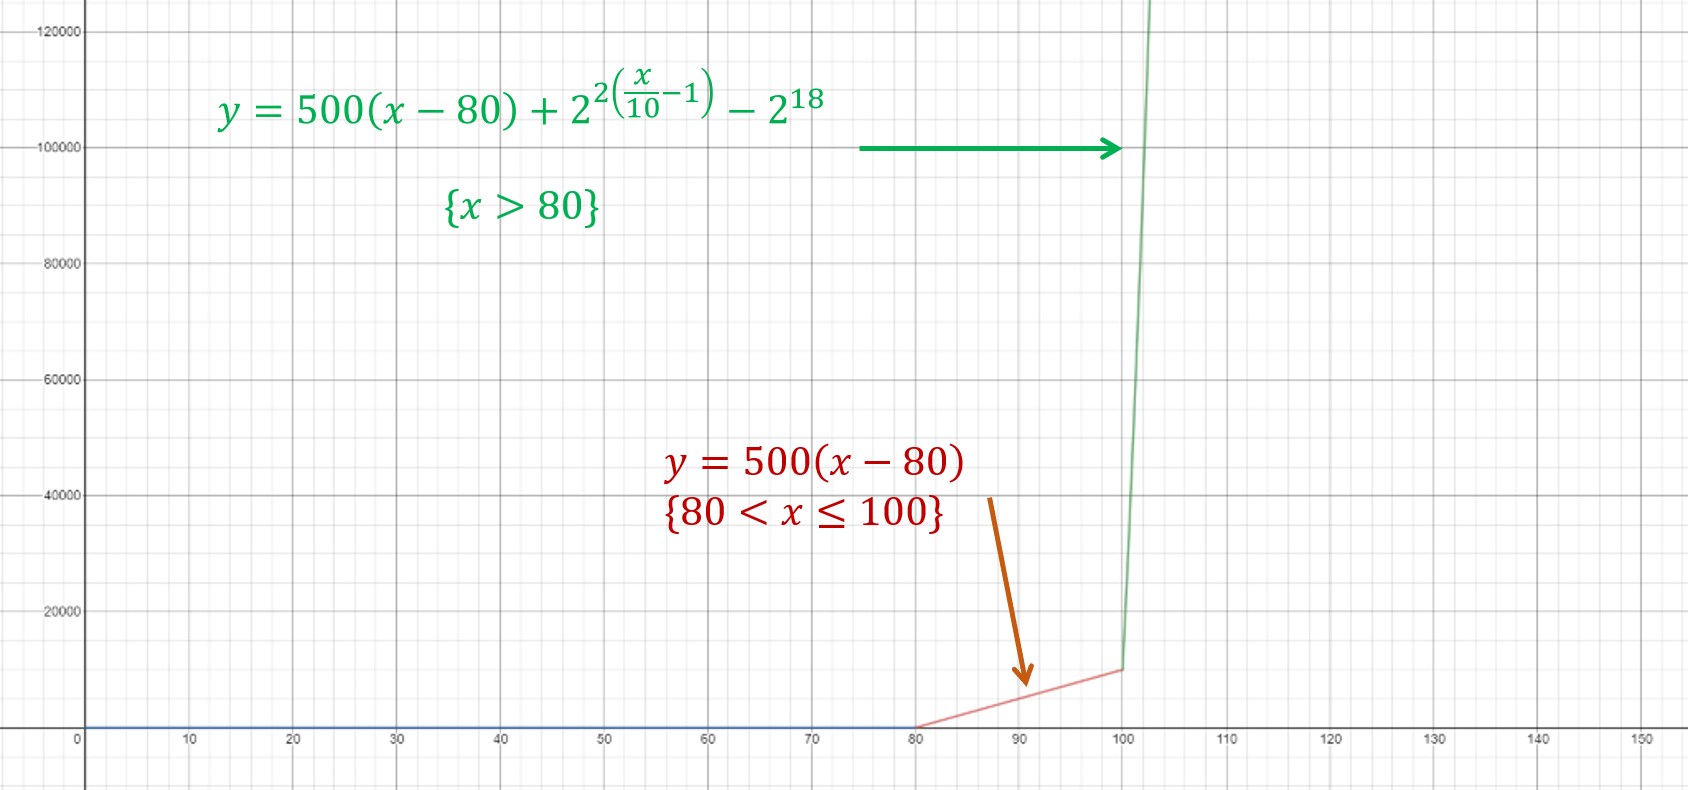
\includegraphics[width=\linewidth]{images/penalty_graph.png}
    \end{center}
    \caption[กราฟแสดงการเพิ่มขึ้นของค่า penalty]{กราฟแสดงการเพิ่มขึ้นของค่า penalty}
    \label{fig:penalty_graph}     
\end{figure}
\newpage
\section{การประเมินระบบโดยสอบถามความพึงพอใจของนักศึกษา}
ตัวชี้วัดที่ใช้ในการคำนวณ penalty ของตารางสอบที่ได้จากระบบนั้น อาจจะไม่ครอบคลุมความพึงประสงค์ทุกรูปแบบจากนักศึกษา หรือน้ำหนักของตัวชี้วัดที่ใช้ในการคำนวณ penalty นั้นอาจจะเป็นไปได้หลายรูปแบบ
\enskip การสอบถามความพึงพอใจของนักศึกษานั้นจะช่วยในการปรับปรุงอัลกอริทึมเพื่อให้สามารถเลือกใช้น้ำหนักของตัวชี้วัดที่เหมาะสมมากขึ้นในการจัดตารางสอบ
อีกทั้งยังช่วยยืนยันว่าตัวชี้วัดที่โปรแกรมใช้คํานวณค่าความเหมาะสมของตารางสอบนั้นสอดคล้องกับความต้องการของผู้ใช้งาน 
\enskip โดยการประเมินระบบด้วยวิธีการนี้นั้นจะมีการแสดงตารางสอบหลายแบบเพื่อให้นักศึกษาได้เปรียบเทียบและ
ให้คะแนนความพึงพอใจกับตารางสอบแบบต่าง ๆ ซึ่งตารางสอบที่ใช้ในแบบสอบถามนั้นจะเป็นตารางสอบของนักศึกษาคนที่ตอบแบบสอบถาม 
โดยเป็นตารางสอบที่มีค่า penalty ต่ำที่สุดที่ได้จากระบบ โดยจะมีตารางสอบหลายแบบที่มีค่าน้ำหนักของตัวชี้วัดที่แตกต่างกันออกไป 
และรวมไปถึงตารางสอบดั้งเดิมของสำนักทะเบียนและประมวลผลด้วย
